\documentclass{standalone}
\usepackage{tikz}
\usetikzlibrary{patterns, positioning}

\begin{document}
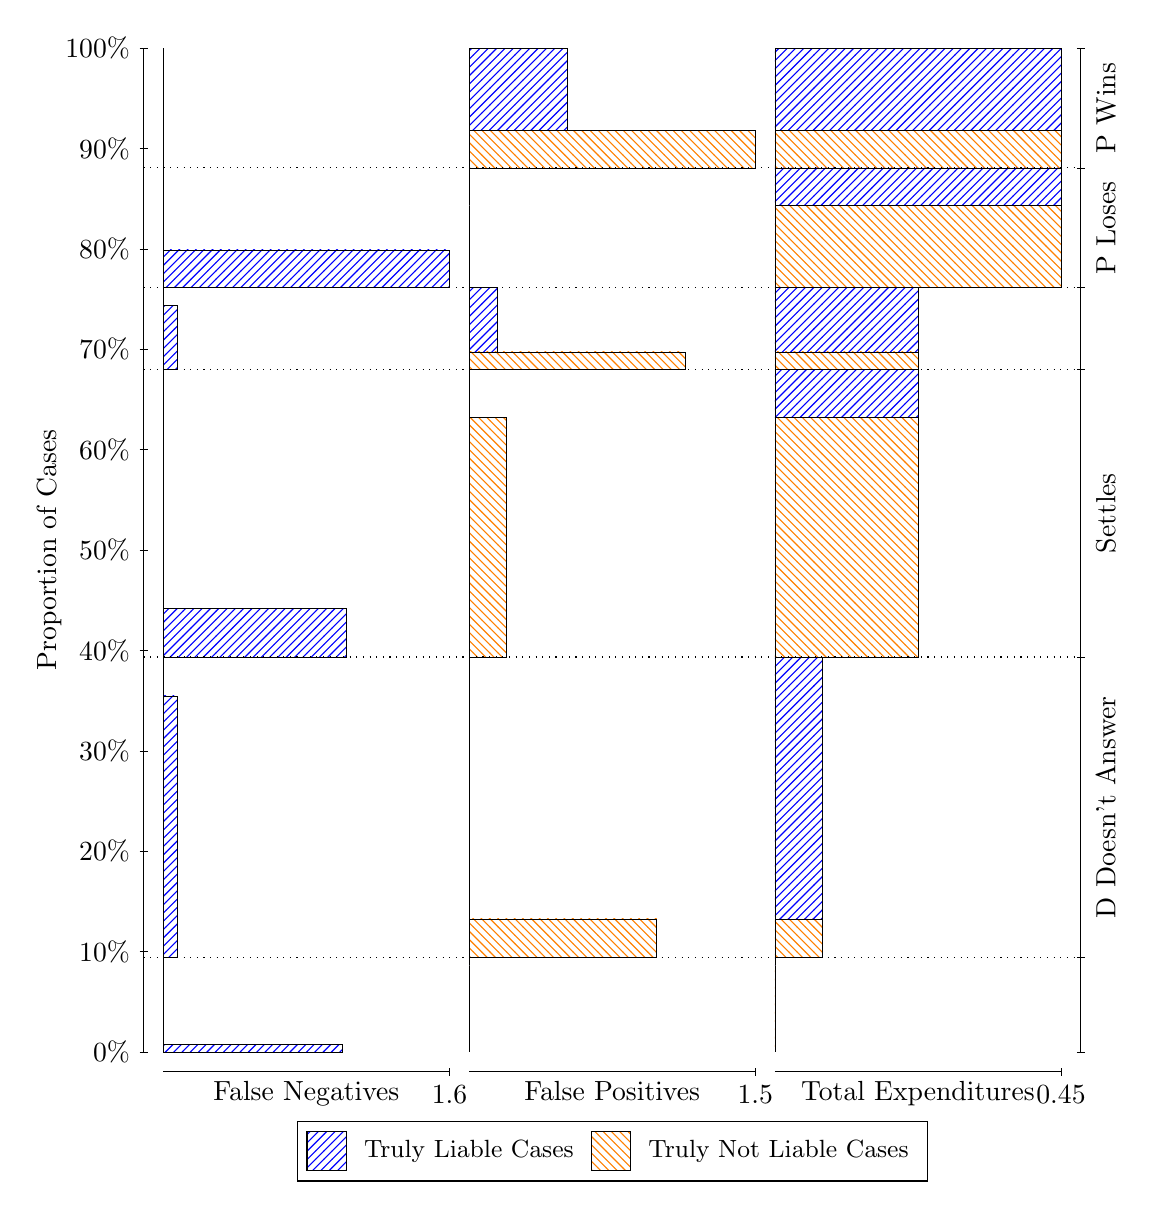
\begin{tikzpicture}
\draw[black, very thin] (1.5,1.75) -- (1.5,14.5);
\node[rotate=90, anchor=center] at (0.3, 8.125) {Proportion of Cases};
\draw[black, very thin] (1.45,1.75) -- (1.55,1.75);
\node[anchor=east] at (1.45, 1.75) {0\%};
\draw[black, very thin] (1.45,3.025) -- (1.55,3.025);
\node[anchor=east] at (1.45, 3.025) {10\%};
\draw[black, very thin] (1.45,4.3) -- (1.55,4.3);
\node[anchor=east] at (1.45, 4.3) {20\%};
\draw[black, very thin] (1.45,5.575) -- (1.55,5.575);
\node[anchor=east] at (1.45, 5.575) {30\%};
\draw[black, very thin] (1.45,6.85) -- (1.55,6.85);
\node[anchor=east] at (1.45, 6.85) {40\%};
\draw[black, very thin] (1.45,8.125) -- (1.55,8.125);
\node[anchor=east] at (1.45, 8.125) {50\%};
\draw[black, very thin] (1.45,9.4) -- (1.55,9.4);
\node[anchor=east] at (1.45, 9.4) {60\%};
\draw[black, very thin] (1.45,10.675) -- (1.55,10.675);
\node[anchor=east] at (1.45, 10.675) {70\%};
\draw[black, very thin] (1.45,11.95) -- (1.55,11.95);
\node[anchor=east] at (1.45, 11.95) {80\%};
\draw[black, very thin] (1.45,13.225) -- (1.55,13.225);
\node[anchor=east] at (1.45, 13.225) {90\%};
\draw[black, very thin] (1.45,14.5) -- (1.55,14.5);
\node[anchor=east] at (1.45, 14.5) {100\%};

\draw[black, very thin] (13.4,1.75) -- (13.4,14.5);
\draw[black, very thin] (13.35,1.75) -- (13.45,1.75);
\node[anchor=west] at (13.35, 1.75) {};
\draw[black, very thin] (13.35,2.9466) -- (13.45,2.9466);
\node[anchor=west] at (13.35, 2.9466) {};
\draw[black, very thin] (13.35,6.7656) -- (13.45,6.7656);
\node[anchor=west] at (13.35, 6.7656) {};
\draw[black, very thin] (13.35,10.421) -- (13.45,10.421);
\node[anchor=west] at (13.35, 10.421) {};
\draw[black, very thin] (13.35,11.456) -- (13.45,11.456);
\node[anchor=west] at (13.35, 11.456) {};
\draw[black, very thin] (13.35,12.978) -- (13.45,12.978);
\node[anchor=west] at (13.35, 12.978) {};
\draw[black, very thin] (13.35,14.5) -- (13.45,14.5);
\node[anchor=west] at (13.35, 14.5) {};

\draw[black, very thin, pattern color=blue, pattern=north east lines] (1.75,1.75) rectangle (4.0208,1.8503);
\draw[black, very thin, pattern color=orange, pattern=north west lines] (1.75,1.8503) rectangle (1.75,2.9466);
\draw[black, very thin, pattern color=blue, pattern=north east lines] (1.75,2.9466) rectangle (1.9203,6.2717);
\draw[black, very thin, pattern color=orange, pattern=north west lines] (1.75,6.2717) rectangle (1.75,6.7656);
\draw[black, very thin, pattern color=blue, pattern=north east lines] (1.75,6.7656) rectangle (4.0776,7.3793);
\draw[black, very thin, pattern color=orange, pattern=north west lines] (1.75,7.3793) rectangle (1.75,10.421);
\draw[black, very thin, pattern color=blue, pattern=north east lines] (1.75,10.421) rectangle (1.9203,11.234);
\draw[black, very thin, pattern color=orange, pattern=north west lines] (1.75,11.234) rectangle (1.75,11.456);
\draw[black, very thin, pattern color=blue, pattern=north east lines] (1.75,11.456) rectangle (5.3833,11.935);
\draw[black, very thin, pattern color=orange, pattern=north west lines] (1.75,11.935) rectangle (1.75,12.978);
\draw[black, very thin, pattern color=orange, pattern=north west lines] (1.75,12.978) rectangle (1.75,13.457);
\draw[black, very thin, pattern color=blue, pattern=north east lines] (1.75,13.457) rectangle (1.75,14.5);
\draw[black, very thin, pattern color=orange, pattern=north west lines] (5.6333,1.75) rectangle (5.6333,2.8463);
\draw[black, very thin, pattern color=blue, pattern=north east lines] (5.6333,2.8463) rectangle (5.6333,2.9466);
\draw[black, very thin, pattern color=orange, pattern=north west lines] (5.6333,2.9466) rectangle (8.0158,3.4404);
\draw[black, very thin, pattern color=blue, pattern=north east lines] (5.6333,3.4404) rectangle (5.6333,6.7656);
\draw[black, very thin, pattern color=orange, pattern=north west lines] (5.6333,6.7656) rectangle (6.1098,9.8071);
\draw[black, very thin, pattern color=blue, pattern=north east lines] (5.6333,9.8071) rectangle (5.6333,10.421);
\draw[black, very thin, pattern color=orange, pattern=north west lines] (5.6333,10.421) rectangle (8.3732,10.642);
\draw[black, very thin, pattern color=blue, pattern=north east lines] (5.6333,10.642) rectangle (5.9907,11.456);
\draw[black, very thin, pattern color=orange, pattern=north west lines] (5.6333,11.456) rectangle (5.6333,12.498);
\draw[black, very thin, pattern color=blue, pattern=north east lines] (5.6333,12.498) rectangle (5.6333,12.978);
\draw[black, very thin, pattern color=orange, pattern=north west lines] (5.6333,12.978) rectangle (9.2667,13.457);
\draw[black, very thin, pattern color=blue, pattern=north east lines] (5.6333,13.457) rectangle (6.8842,14.5);
\draw[black, very thin, pattern color=orange, pattern=north west lines] (9.5167,1.75) rectangle (9.5167,2.8463);
\draw[black, very thin, pattern color=blue, pattern=north east lines] (9.5167,2.8463) rectangle (9.5167,2.9466);
\draw[black, very thin, pattern color=orange, pattern=north west lines] (9.5167,2.9466) rectangle (10.122,3.4404);
\draw[black, very thin, pattern color=blue, pattern=north east lines] (9.5167,3.4404) rectangle (10.122,6.7656);
\draw[black, very thin, pattern color=orange, pattern=north west lines] (9.5167,6.7656) rectangle (11.333,9.8071);
\draw[black, very thin, pattern color=blue, pattern=north east lines] (9.5167,9.8071) rectangle (11.333,10.421);
\draw[black, very thin, pattern color=orange, pattern=north west lines] (9.5167,10.421) rectangle (11.333,10.642);
\draw[black, very thin, pattern color=blue, pattern=north east lines] (9.5167,10.642) rectangle (11.333,11.456);
\draw[black, very thin, pattern color=orange, pattern=north west lines] (9.5167,11.456) rectangle (13.15,12.498);
\draw[black, very thin, pattern color=blue, pattern=north east lines] (9.5167,12.498) rectangle (13.15,12.978);
\draw[black, very thin, pattern color=orange, pattern=north west lines] (9.5167,12.978) rectangle (13.15,13.457);
\draw[black, very thin, pattern color=blue, pattern=north east lines] (9.5167,13.457) rectangle (13.15,14.5);
\draw[black, dotted] (1.5,2.9466) -- (13.4,2.9466);
\draw[black, dotted] (1.5,6.7656) -- (13.4,6.7656);
\draw[black, dotted] (1.5,10.421) -- (13.4,10.421);
\draw[black, dotted] (1.5,11.456) -- (13.4,11.456);
\draw[black, dotted] (1.5,12.978) -- (13.4,12.978);
\draw[black, very thin] (1.75,1.5) -- (5.3833,1.5);
\node[anchor=north] at (3.5667, 1.5) {False Negatives};
\draw[black, very thin] (5.3833,1.45) -- (5.3833,1.55);
\node[anchor=north] at (5.3833, 1.45) {1.6};

\draw[black, very thin] (5.6333,1.5) -- (9.2667,1.5);
\node[anchor=north] at (7.45, 1.5) {False Positives};
\draw[black, very thin] (9.2667,1.45) -- (9.2667,1.55);
\node[anchor=north] at (9.2667, 1.45) {1.5};

\draw[black, very thin] (9.5167,1.5) -- (13.15,1.5);
\node[anchor=north] at (11.333, 1.5) {Total Expenditures};
\draw[black, very thin] (13.15,1.45) -- (13.15,1.55);
\node[anchor=north] at (13.15, 1.45) {0.45};


\node[black, centered, rotate=90] at (13.72, 4.8561) {D Doesn't Answer};
\node[black, centered, rotate=90] at (13.72, 8.5932) {Settles};

\node[black, centered, rotate=90] at (13.72, 12.217) {P Loses};
\node[black, centered, rotate=90] at (13.72, 13.739) {P Wins};

\draw (7.449999999999999,1.5) node[draw=none] (baseCoordinate) {};
\begin{scope}[align=center]
        \matrix[scale=0.5, draw=black, below=0.5cm of baseCoordinate, nodes={draw}, column sep=0.1cm]{
            \node[rectangle, draw, minimum width=0.5cm, minimum height=0.5cm, pattern=north east lines, pattern color=blue] {}; &
            \node[draw=none, font=\small] (B) {Truly Liable Cases}; &
            \node[rectangle, draw, minimum width=0.5cm, minimum height=0.5cm, pattern=north west lines, pattern color=orange] {}; &
            \node[draw=none, font=\small] (B) {Truly Not Liable Cases}; \\
            };
\end{scope}

\end{tikzpicture}
\end{document}